\subsection{Perplexity Analysis of Extracted Traces}\label{app:ppl}

Behavioral similarity does not by itself imply memorization. We further study whether open-weight models assign unusually low perplexity to decoded proprietary traces, and whether they can reproduce those traces verbatim?

\subsubsection{Probabilistic Extraction of Reasoning Traces}\label{app:npextract}

We first investigate whether the open-weight models can reproduce short spans of the decoded reasoning traces \emph{verbatim}.

\paragraph{Setting.} We follow the probabilistic-extraction framework of \citet{hayes2025measuring}. For a target span \(z\) of \(k\) tokens, one teacher-forcing pass gives the probability \(p_z\) that a temperature-\(1\) sample reproduces the span exactly. The probability of extracting the span within \(n\) independent queries is
\[
P(\text{extract within }n\text{ queries})
    = 1-(1-p_z)^n.
\]
We score target spans in the reasoning channel. Unless stated otherwise, we use \(k=16\) and report medians across problems.

\paragraph{Model Details.} Throughout this section, we use GLM-5.2, GPT-OSS-120B, Kimi-K2.6, and Kimi-K2.7-Code through Fireworks; Inkling through Tinker (Thinking Machines); and Kimi-K3 and DeepSeek-V4-Flash through Parasail. We use these models to score prompts and reasoning traces at the token level. To obtain each scorer's native reasoning traces, we sample through OpenRouter at temperature \(1.0\), with completion budgets of up to \(131{,}000\) tokens. We note that serving differences are an important limitation here. For example, running Kimi-K3 at full precision requires an eight-GPU B300 node. We therefore cannot fully control for differences in model implementations or other provider-specific effects. These differences may substantially affect the reported perplexities.


\paragraph{Data.} We use the 30 HLE problems from \Cref{app:prefill_qualitative}, evenly split between STEM and non-STEM, together with their decoded Opus-4.8 reasoning traces and visible answers. We also use 10 AIME25 problems for which the decoded reasoning for both GPT-5.6 Sol and Opus 4.8 has low reconstruction error. As controls, we sample one native reasoning trace and visible answer from every scorer for each problem. We generate these traces at temperature \(1.0\) under the same chat template later used for scoring.

\paragraph{Results.}

\Cref{fig:np_hle,fig:np_aime} show the cumulative probability of reproducing the next \(k=16\) target tokens verbatim as the number of sampling attempts increases. Results are reported as medians across the 30 HLE problems for decoded Opus~4.8 traces and across the 10 AIME~2025 problems for decoded GPT-5.6 Sol and Opus~4.8 traces.

When conditioned only on the problem, none of the evaluated models provides evidence of practical verbatim memorization of the decoded reasoning traces. Kimi-K3 yields the highest extraction probabilities, but reproducing a 16-token reasoning span would still require on the order of \(10^{10}\) queries on HLE and, on AIME~2025, between \(10^{9}\) and \(10^{12}\) queries depending on whether the target is the decoded Opus~4.8 or the GPT-5.6 Sol trace.

On HLE, conditioning the models on the first \(1\%\) of the decoded Opus~4.8 reasoning increases the probability of reproducing the subsequent reasoning span, but leaves it far outside any practical query budget. The median requirement drops from \(10^{14}\) to \(10^{11}\) queries for GLM-5.2, while for Kimi-K2.6 and Kimi-K3 it stays at roughly \(10^{11}\) and \(10^{10}\). Kimi-K3 thus remains the most extractable of the three in absolute terms, four to six orders of magnitude below DeepSeek-V4-Flash and Inkling (\(10^{14}\) and \(10^{16}\)). The ordering across models is nonetheless consistent with the reasoning-drift analysis in \Cref{app:reasoning_drift}, which shows that Kimi-K3, Kimi-K2.6, and GLM-5.2 more readily continue reasoning in the style of Opus~4.8 and GPT-5.6 Sol.

The visible answer is far cheaper to extract than the reasoning, and it is here that the models differ. For HLE, Kimi-K3 requires approximately \(4\times10^{5}\) queries to reproduce the next 16 tokens of the Opus~4.8 answer when conditioned on a \(1\%\) reasoning prefill, and approximately \(10^{5}\) queries when conditioned on the complete decoded reasoning trace. GLM-5.2 and Kimi-K2.6 are the next most extractable models under this evaluation (median \({\sim}10^{7}\) and \({\sim}10^{9}\) queries with the complete trace), whereas Inkling and DeepSeek-V4-Flash require more than \(10^{14}\) queries in either condition. On AIME~2025, a 16-token span of the GPT-5.6 Sol visible answer can be reproduced by Kimi-K3 in as few as \(10^{2}\) queries when conditioned on Kimi-K3's own reasoning for the same problem. We do not observe a comparable effect for the other evaluated models. These visible-answer results support the output-drift findings in \Cref{app:output_drift}.

Overall, the current results do not support direct verbatim memorization of the decoded traces, and a short reasoning prefill moves the reasoning channel itself only modestly. The effect is concentrated in the visible answer: relative to conditioning on their own reasoning, having the source trace in context lowers the cost of reproducing the Opus~4.8 answer by roughly \(13\) orders of magnitude for Kimi-K3 and GLM-5.2, against \(3\) for Kimi-K2.6. This suggests that Kimi-K3 and GLM-5.2 are unusually likely to continue the visible-answer patterns induced by the source-model trace.

\begin{figure}[H]
\centering
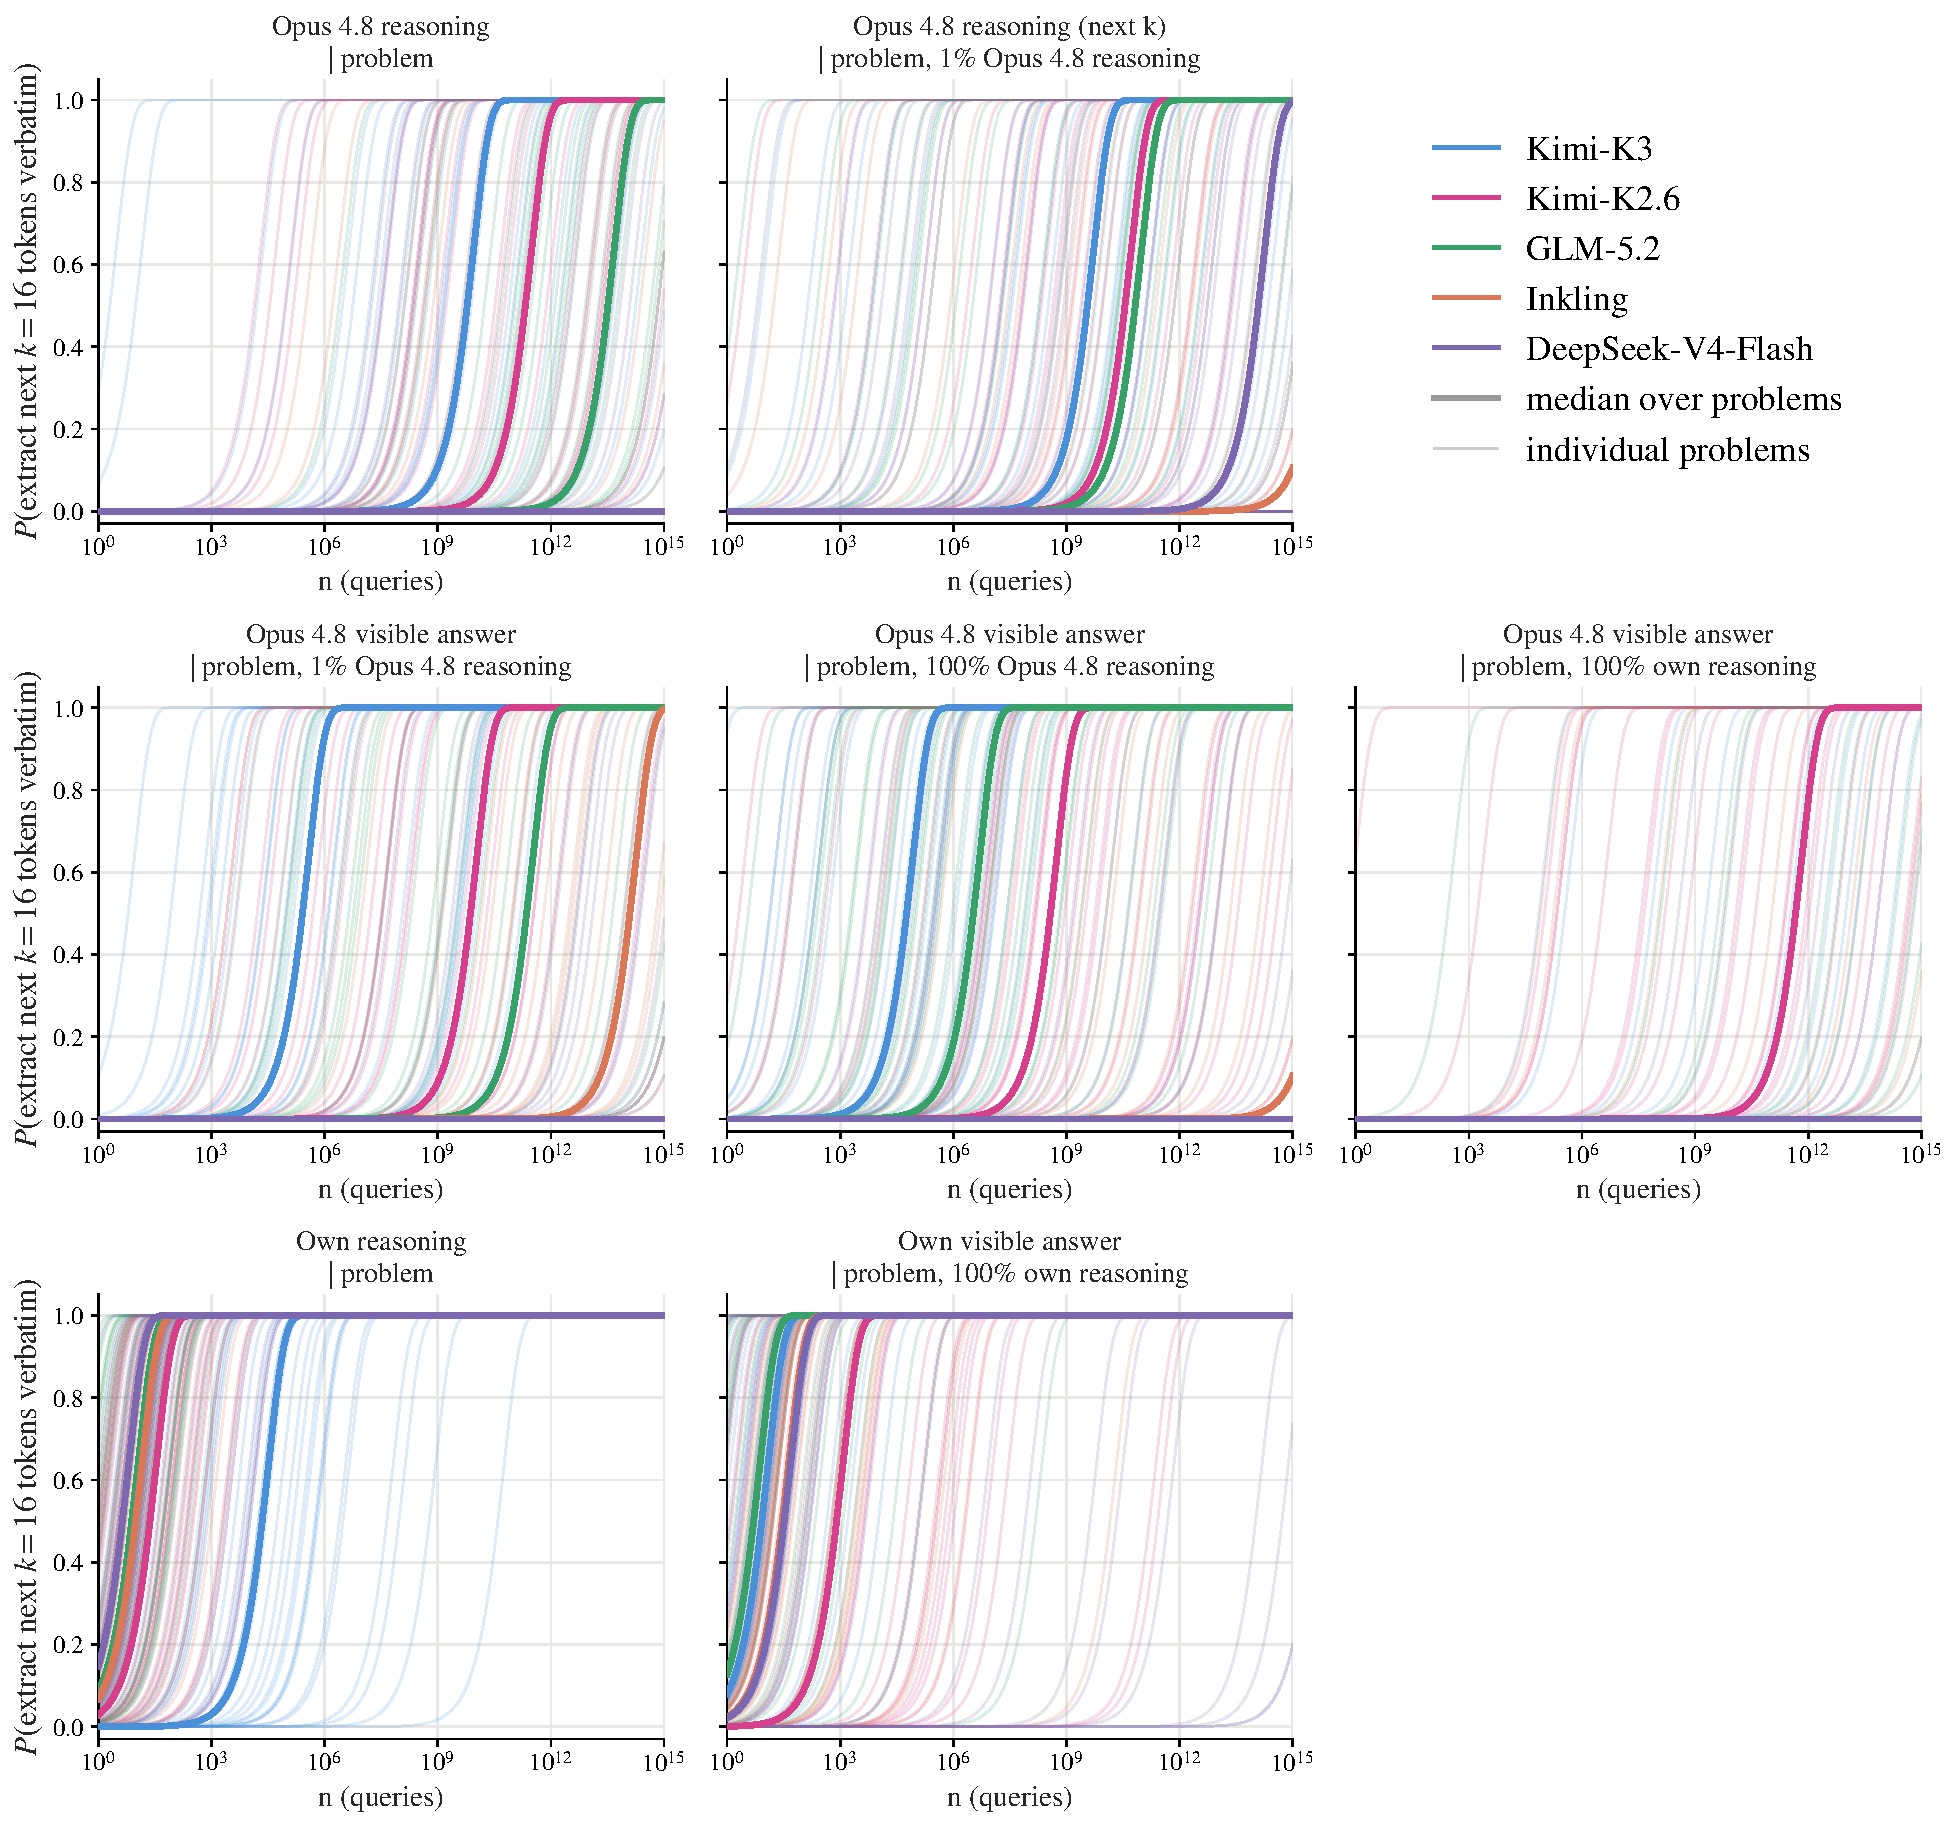
\includegraphics[width=\linewidth]{figures/np_extraction/hle.pdf}
\caption{Probabilistic extraction \citep{hayes2025measuring} of reasoning traces on $30$ HLE problems, $k=16$ tokens, median over problems (faint lines: individual problems). Rows: extraction of reasoning; extraction of the visible answer under increasing context; the scorer's own trace as control.}
\label{fig:np_hle}
\end{figure}

\begin{figure}[H]
\centering
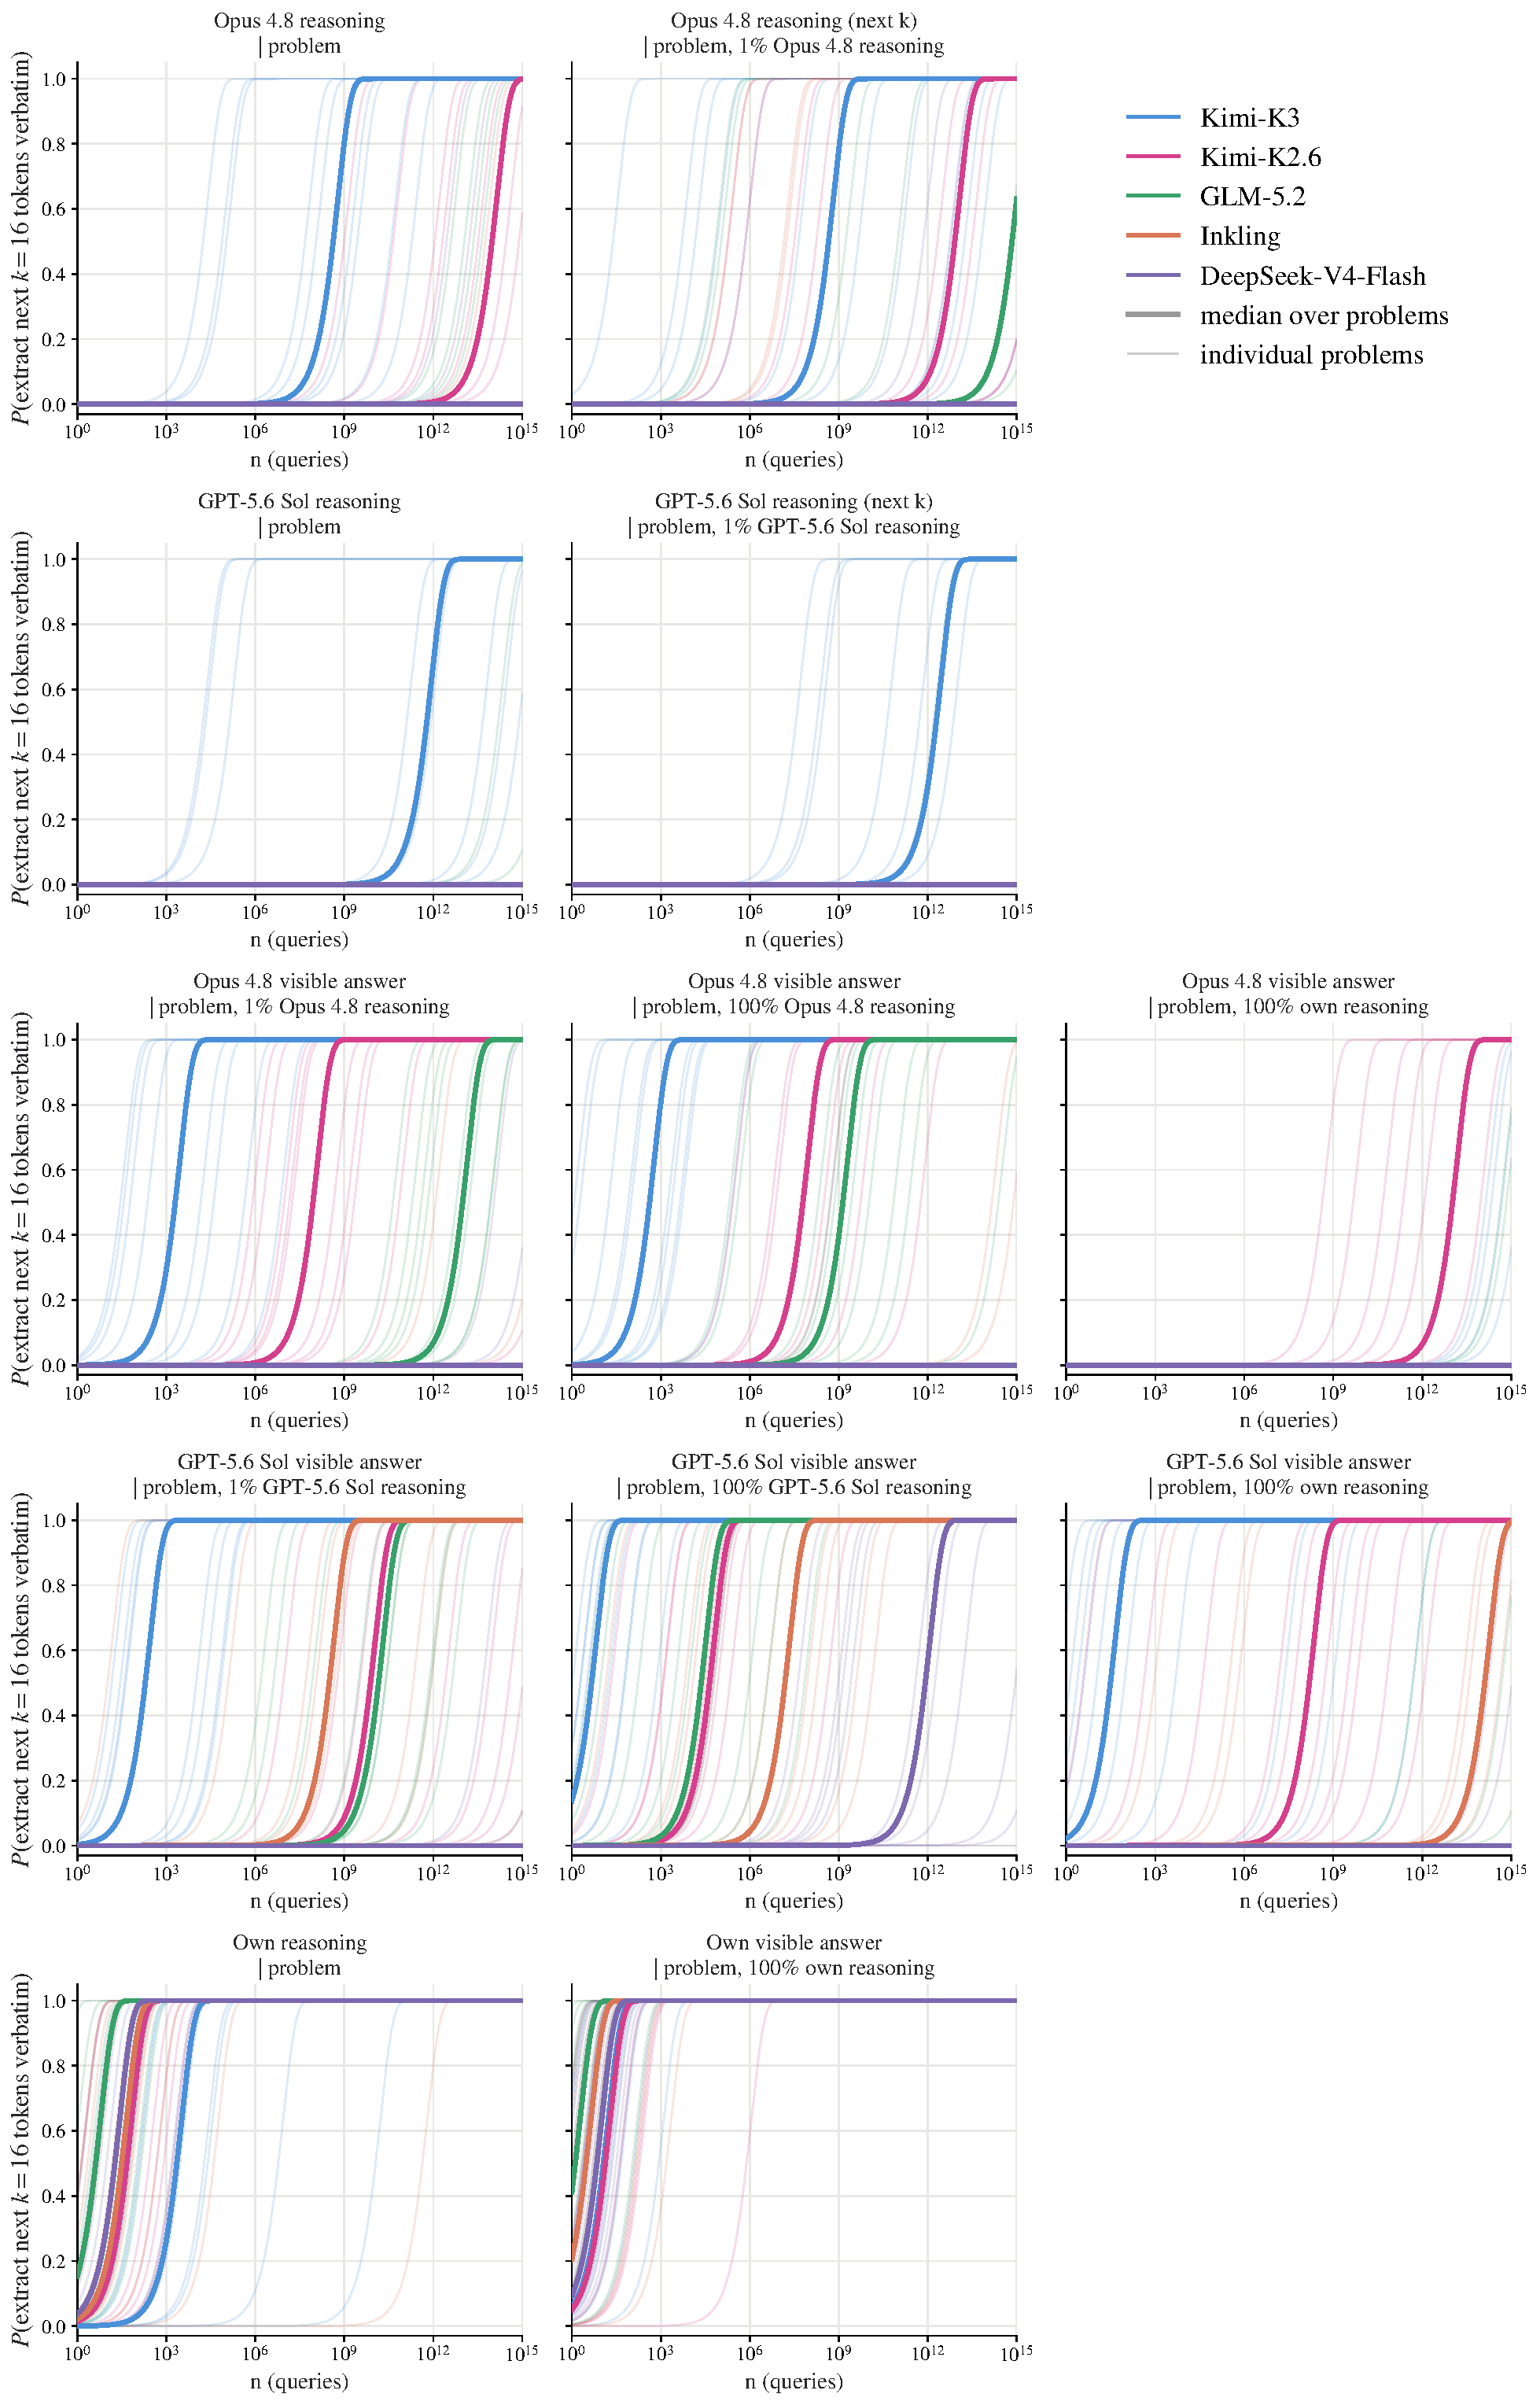
\includegraphics[width=\linewidth]{figures/np_extraction/aime.pdf}
\caption{As in \Cref{fig:np_hle}, on $10$ AIME 2025 problems, with GPT-5.6 Sol decoded traces as a second prefill. Kimi-K3 reaches GPT-5.6 Sol's answer wording within ${\sim}10^{2}$ queries even conditioned on its own reasoning (third row, right), while no other model does so within $10^{8}$ queries.}
\label{fig:np_aime}
\end{figure}

\subsubsection{Perplexity of Reasoning Traces}\label{app:ppl_traces}

Exact extraction tests whether a model can reproduce a short target span. We next test a broader question: Which reasoning traces does each scorer treat as native, in terms of perplexity?

\paragraph{Setting.}
%For a reasoning trace t associated with problem q, we render the scorer's native chat template up to the beginning of the reasoning channel, append the tokens of t, and obtain the conditional log-probability of each trace token. We report perplexity over reasoning tokens only: $\mathrm{PPL}(t\mid q)=\exp\!\big(-\tfrac1{|t|}\sum_i \log p(t_i\mid q, t_{<i})\big)$.
%paragraph{Setting.}
For a reasoning trace \(t\) associated with problem \(q\), we render the scorer's native chat template up to the start of the reasoning channel and append the tokens of \(t\). We then compute the conditional log-probability of every reasoning token. We report perplexity over the reasoning tokens only. Formally,
\[
\mathrm{PPL}(t\mid q)
=
\exp\!\left(
-\frac{1}{|t|}
\sum_i
\log p(t_i\mid q,t_{<i})
\right)
\]
We use the same model details as the preceding section.

\paragraph{Experimental Details.} We use the same 120 Codeforces problems as in \Cref{fig:teaser}. For each open-weight model, we generate native reasoning traces and score them under every other open-weight scorer. For proprietary models, we place the original problem in the user turn and the target trace in the reasoning channel of the scorer's chat template. We also score the decoded traces used in \Cref{fig:teaser}, which were recovered using the procedure in \Cref{sec:extraction}. We retain only traces whose decoded-to-billed thinking-token ratio \(r\) satisfies $\mid 1−r \mid <0.05$. We use the same model details as the above section.

%We generate reasoning traces for the same 120 Codeforces programming problems used in \Cref{fig:teaser}. For each open-source model, we generate native reasoning traces and subsequently score them under the other open-source models by placing the original problem in the user turn and the trace in the reasoning turn of the scorer's chat template. For decoded traces from \Cref{fig:teaser}, obtained using the procedure described in \Cref{sec:extraction}, we retain only those for which the decoded-to-billed thinking-token ratio r satisfies $\mid 1−r \mid <0.05$. We use the same model details as the above section.

\begin{figure}[H]
\centering
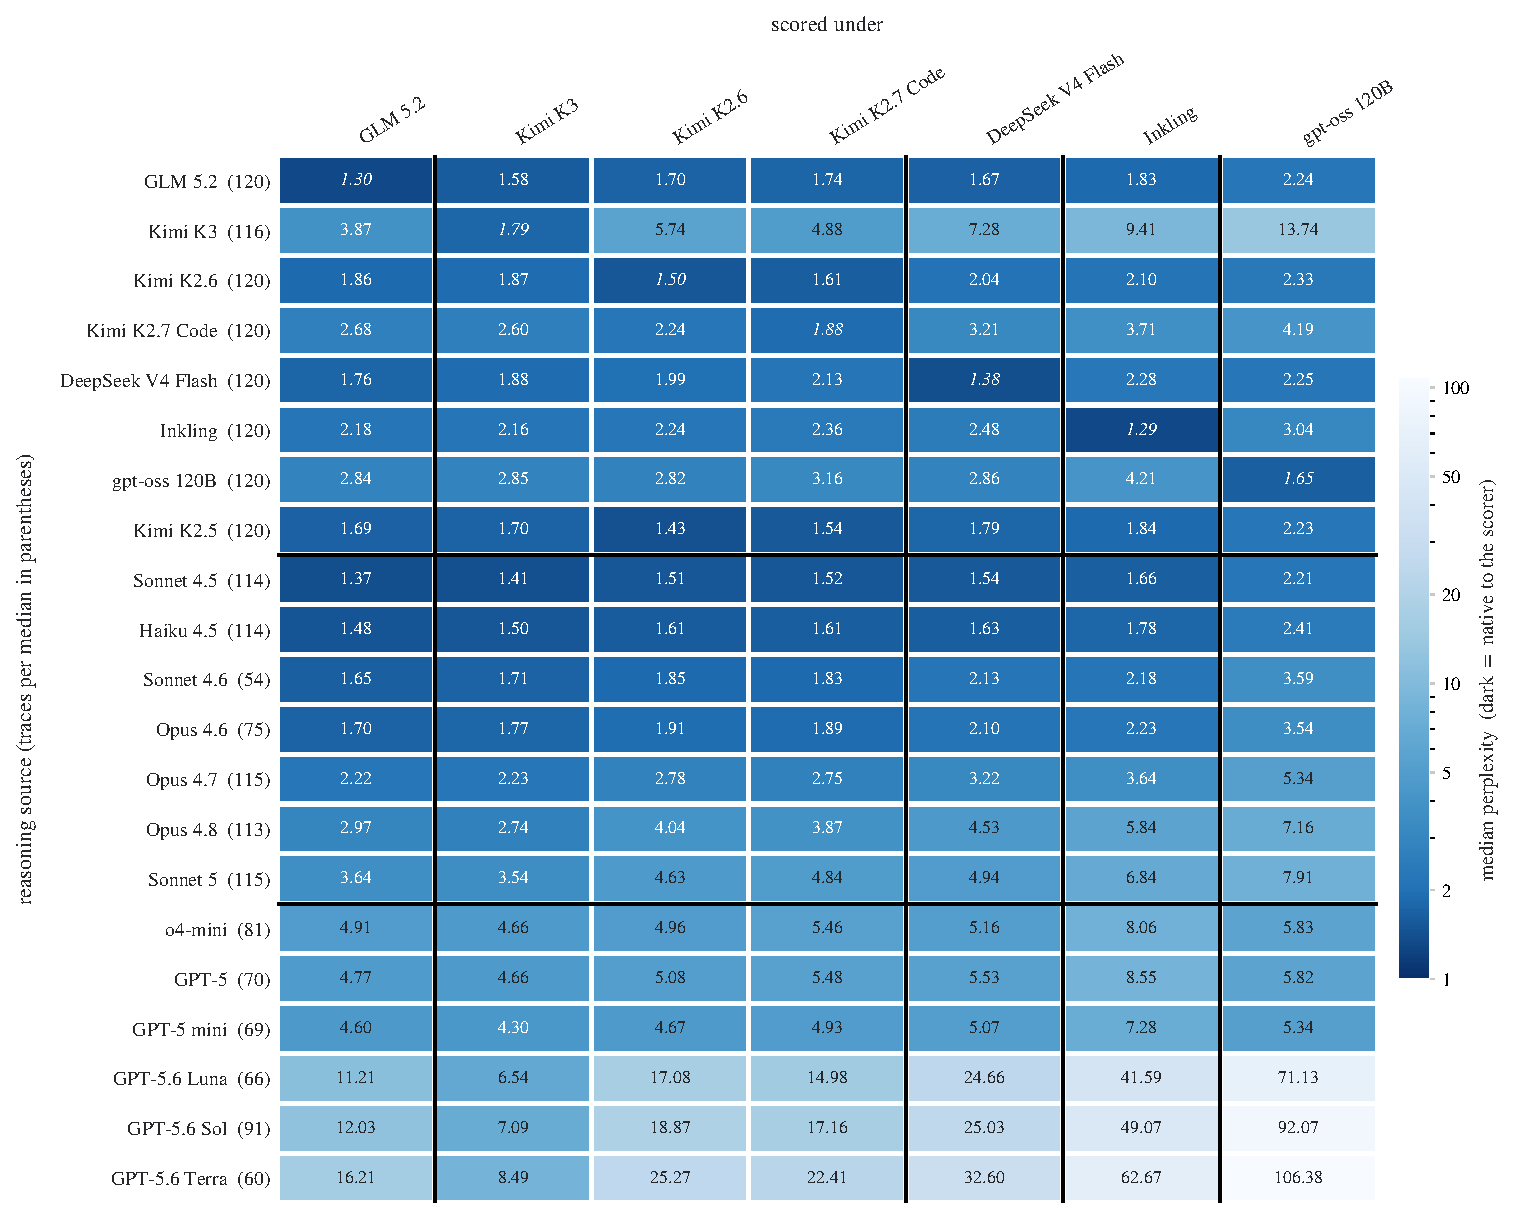
\includegraphics[width=\linewidth]{figures/prefill_ppl/ppl_heatmap.pdf}
\caption{\textbf{Median perplexity of reasoning traces under seven scoring models.} Every model scores perplexity of the reasoning,
conditional on the problem, over the same 120 Codeforces problems. Rows are the
model whose reasoning is being scored; columns are the model doing the scoring. The diagonal, where a model scores its own reasoning, is set in italic. Colour is on a logarithmic scale, dark for reasoning the scorer finds native.}
\label{fig:ppl_heatmap}
\end{figure}


\paragraph{Results.}  We observe a few surprising findings. First, every model except Kimi-K3 and Kimi-K2.7-Code, assigns significantly higher average perplexity to its own reasoning than to reasoning from other models. Thus, a model's native trace is not generally the trace it considers most probable.

Decoded reasoning from Sonnet-4.5 and Haiku-4.5 has relatively high average perplexity under every scorer. Under GLM-5.2, the four reasoning sources with perplexities closest to GLM-5.2's own reasoning are four consecutive Anthropic model releases. However, perplexity is a coarse metric that may not capture fine-grained distributional fit, and hence results should not be interpreted as a confirmatory measure of model similarity.